% This file was created by tikzplotlib v0.9.1.
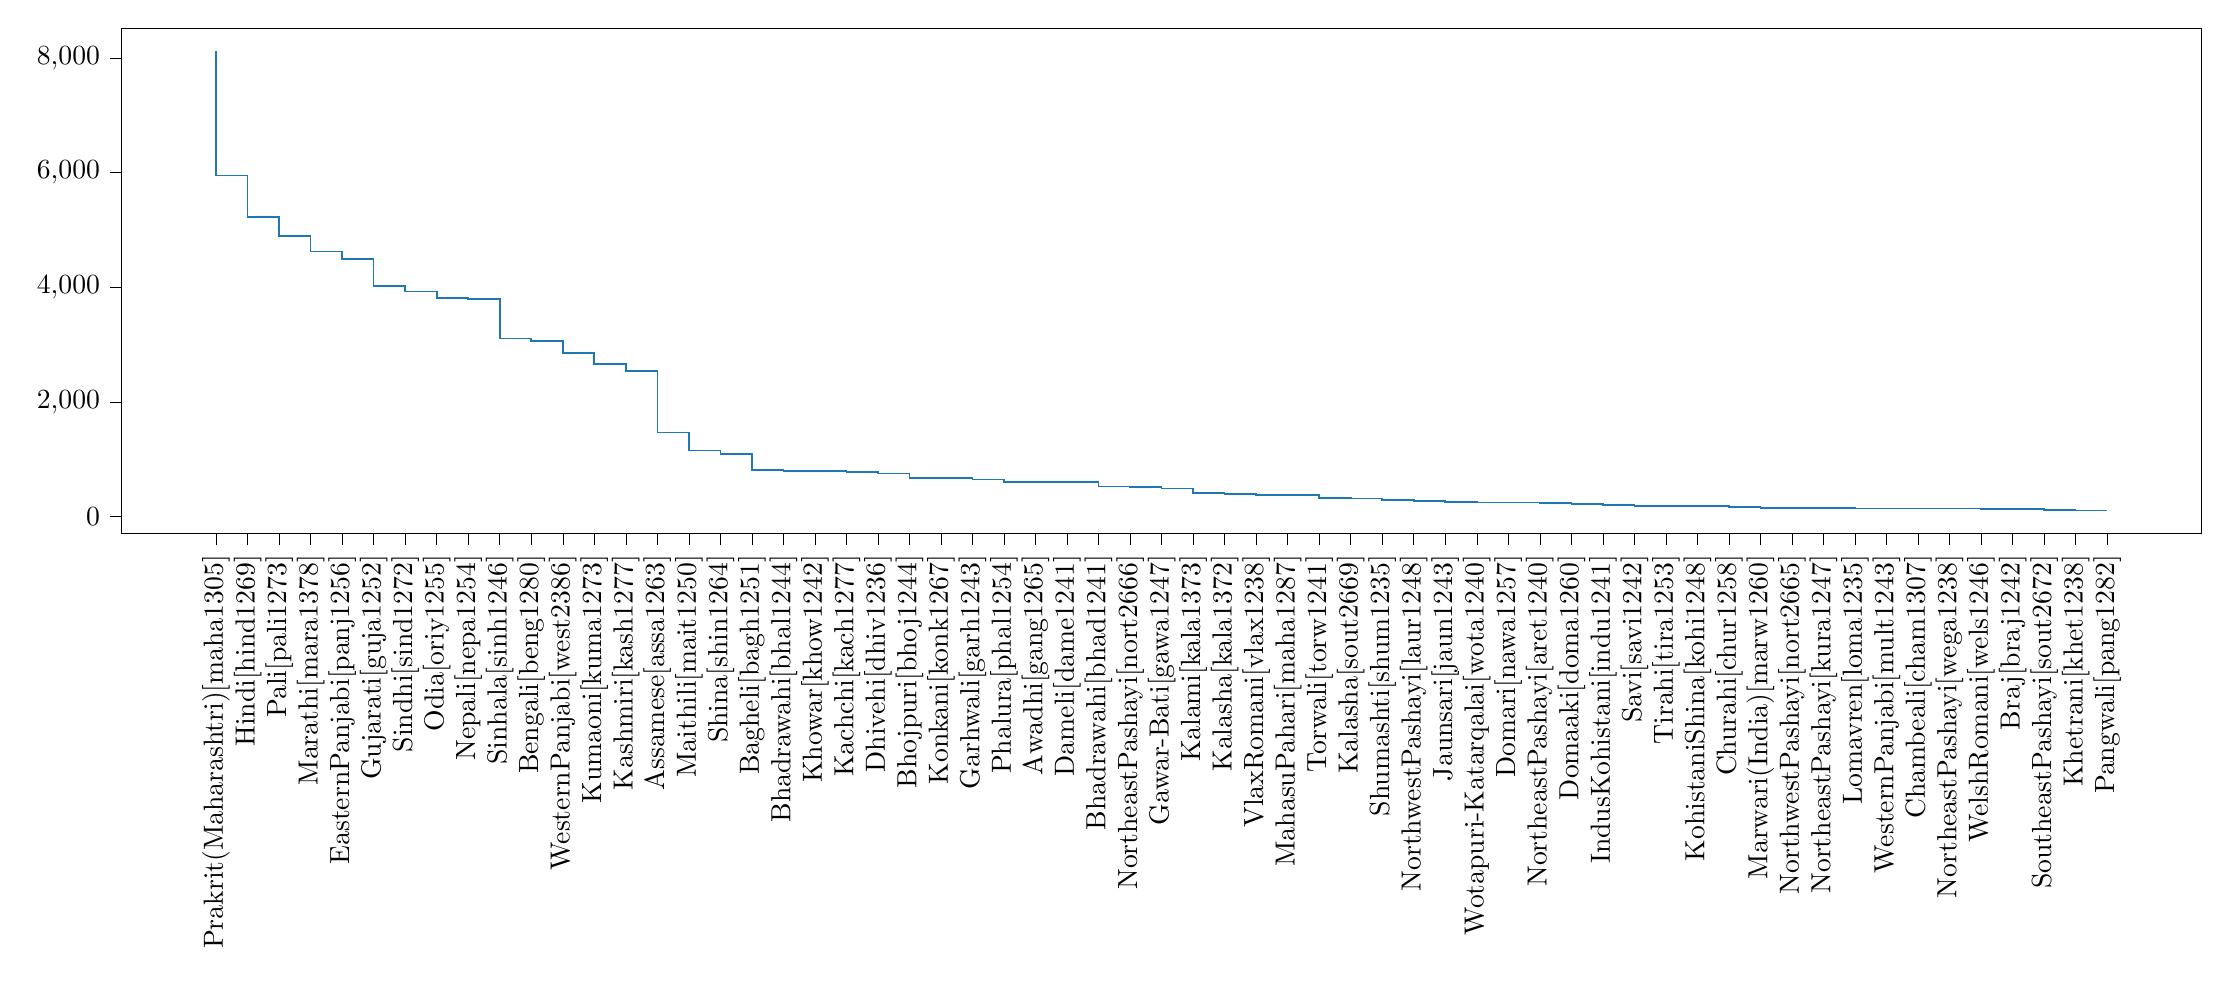
\begin{tikzpicture}

\definecolor{color0}{rgb}{0.12156862745098,0.466666666666667,0.705882352941177}

\begin{axis}[
height=8cm,
tick align=outside,
tick pos=left,
width=28cm,
x grid style={white!69.0196078431373!black},
xmin=-3, xmax=63,
xtick style={color=black},
xtick={0,1,2,3,4,5,6,7,8,9,10,11,12,13,14,15,16,17,18,19,20,21,22,23,24,25,26,27,28,29,30,31,32,33,34,35,36,37,38,39,40,41,42,43,44,45,46,47,48,49,50,51,52,53,54,55,56,57,58,59,60},
xticklabel style = {rotate=90.0},
xticklabels={Prakrit(Maharashtri)[maha1305],Hindi[hind1269],Pali[pali1273],Marathi[mara1378],EasternPanjabi[panj1256],Gujarati[guja1252],Sindhi[sind1272],Odia[oriy1255],Nepali[nepa1254],Sinhala[sinh1246],Bengali[beng1280],WesternPanjabi[west2386],Kumaoni[kuma1273],Kashmiri[kash1277],Assamese[assa1263],Maithili[mait1250],Shina[shin1264],Bagheli[bagh1251],Bhadrawahi[bhal1244],Khowar[khow1242],Kachchi[kach1277],Dhivehi[dhiv1236],Bhojpuri[bhoj1244],Konkani[konk1267],Garhwali[garh1243],Phalura[phal1254],Awadhi[gang1265],Dameli[dame1241],Bhadrawahi[bhad1241],NortheastPashayi[nort2666],Gawar-Bati[gawa1247],Kalami[kala1373],Kalasha[kala1372],VlaxRomani[vlax1238],MahasuPahari[maha1287],Torwali[torw1241],Kalasha[sout2669],Shumashti[shum1235],NorthwestPashayi[laur1248],Jaunsari[jaun1243],Wotapuri-Katarqalai[wota1240],Domari[nawa1257],NortheastPashayi[aret1240],Domaaki[doma1260],IndusKohistani[indu1241],Savi[savi1242],Tirahi[tira1253],KohistaniShina[kohi1248],Churahi[chur1258],Marwari(India)[marw1260],NorthwestPashayi[nort2665],NortheastPashayi[kura1247],Lomavren[loma1235],WesternPanjabi[mult1243],Chambeali[cham1307],NortheastPashayi[wega1238],WelshRomani[wels1246],Braj[braj1242],SoutheastPashayi[sout2672],Khetrani[khet1238],Pangwali[pang1282]},
y grid style={white!69.0196078431373!black},
ymin=-297.75, ymax=8518.75,
ytick style={color=black}
]
\addplot [semithick, color0, const plot mark right]
table {%
0 8118
1 5948
2 5225
3 4895
4 4622
5 4490
6 4020
7 3925
8 3807
9 3791
10 3109
11 3060
12 2857
13 2659
14 2543
15 1466
16 1152
17 1086
18 814
19 797
20 789
21 775
22 750
23 672
24 672
25 648
26 607
27 607
28 602
29 525
30 520
31 488
32 407
33 397
34 381
35 374
36 329
37 316
38 292
39 269
40 258
41 245
42 243
43 239
44 224
45 207
46 186
47 186
48 181
49 166
50 148
51 147
52 146
53 143
54 142
55 140
56 138
57 135
58 130
59 120
60 103
};
\end{axis}

\end{tikzpicture}
